\documentclass[conference]{IEEEtran}
\IEEEoverridecommandlockouts
% Template version as of 6/27/2024.

\usepackage{cite}
\usepackage{amsmath,amssymb,amsfonts}
\usepackage{graphicx}
\usepackage{textcomp}
\usepackage{xcolor}

\def\BibTeX{{\rm B\kern-.05em{\sc i\kern-.025em b}\kern-.08em
    T\kern-.1667em\lower.7ex\hbox{E}\kern-.125emX}}

\begin{document}

\title{Building a Vietnamese Secondary Informatics AI Tutor Benchmark
from Teacher-Authored Dialogues}

\author{\IEEEauthorblockN{Author names pending confirmation}
\IEEEauthorblockA{\textit{Affiliations pending confirmation}\\
Vietnam}}

\maketitle

\begin{abstract}
Evaluating a large language model as a tutor requires more than checking
answer correctness: the model must interpret the learner's state, select an
appropriate pedagogical move, and provide calibrated support. We present a
traceable pipeline for constructing a Vietnamese Grades~6--9 Informatics
AI-tutor benchmark from 1,050 teacher-authored dialogues. The pipeline audits
the raw dialogues, establishes a measurement foundation of six pedagogical
principles and six tutor capabilities, and converts every eligible tutor turn
into a context-conditioned next-response candidate. It yields 2,028 candidates
from 665 retained dialogue families. A grounded LLM scores the necessity of
all six principles for each candidate; deterministically checks then identify
1,400 candidates across 655 families that can proceed without targeted review.
We further define an evaluation framework that provides the required
principles to the tutor model, preserves native multi-turn roles, and compares
the generated response with the teacher-authored response using four common
criteria, three criteria per required principle, and criterion-level
Win/Tie/Lose judgments. This work provides a curriculum-grounded construction
and evaluation protocol for Vietnamese Informatics tutoring.
\end{abstract}

\begin{IEEEkeywords}
AI tutoring, benchmark construction, pedagogical evaluation, large
language models, Informatics education, Vietnamese education
\end{IEEEkeywords}

\section{Introduction}

Large language models (LLMs) are increasingly capable of producing
correct answers and fluent explanations, but these abilities do not by
themselves establish that a model can tutor effectively. Tutoring also
requires \textit{(i)} interpreting what a learner currently understands;
\textit{(ii)} diagnosing errors when evidence permits;
\textit{(iii)} selecting an appropriate pedagogical move;
\textit{(iv)} calibrating the amount of support; and
\textit{(v)} communicating in a way that preserves the learner's
opportunity to think. Recent tutoring benchmarks
support this distinction. MathTutorBench reports that mathematical
problem-solving ability does not directly translate into pedagogical
quality \cite{macina2025mathtutorbench}; KMP-Bench separates verifiable
mathematical skills from principle-guided dialogue quality
\cite{shi2026kmpbench}; and TutorBench evaluates responses with
fine-grained, sample-specific criteria \cite{srinivasa2025tutorbench}.
Evaluating a tutor is therefore an assessment-design problem rather than
only a question-answering problem.

Prior AI-tutoring benchmarks leave three gaps for our target setting.
First, their domain coverage is concentrated in mathematics or broad
STEM curricula, while specialized school subjects remain less explored.
Second, they operate predominantly in English, leaving language- and
curriculum-specific tutoring behavior underrepresented. Third, data
construction is not unified: \textit{(i)} KMP-Bench builds pedagogically
planned dialogue flows; \textit{(ii)} TutorBench uses expert-authored
situations and rubrics; and \textit{(iii)} MathTutorBench assembles
existing tutoring datasets under predefined tasks and metrics. In each
case, prior assumptions about tasks or
pedagogical situations structure the data before evaluation. Less is
known about starting from ordinary, teacher-authored pedagogical
dialogues collected independently of a benchmark taxonomy and converting
them into traceable evaluation units.

We address these gaps by constructing a Vietnamese secondary-school
Informatics AI-tutor benchmark for Grades~6--9. Rather than generating
conversations from predefined benchmark situations, our construction and
evaluation process:
\begin{itemize}
    \item begins with raw teacher-authored dialogues and audits their
    structural, curricular, and pedagogical quality;
    \item converts eligible tutor turns into traceable,
    context-conditioned next-response candidate samples;
    \item scores the requirement of all six pedagogical principles for
    every candidate, then applies deterministic filtering and locking
    rules to construct the completed benchmark set; and
    \item combines Allison and Tharby's six pedagogical principles
    \cite{allison2015making} with six tutor capabilities to construct
    context-specific rubrics and an AI-tutor evaluation protocol.
\end{itemize}

The paper makes three contributions:
\begin{enumerate}
    \item an automated and traceable construction pipeline that transforms
    raw teacher-authored dialogues into benchmark candidates and then
    completed benchmark samples through auditing, pedagogical-principle
    assignment, deterministic filtering, and locking;
    \item a context-specific rubric library and evaluation method that
    combines common criteria with criteria associated with each required
    pedagogical principle to evaluate AI tutors; and
    \item a Vietnamese Grades~6--9 Informatics tutoring benchmark
    comprising 1,400 completed samples across 655 raw dialogues.
\end{enumerate}
Together, these contributions establish a curriculum-grounded and
traceable basis for evaluating AI tutoring responses in Vietnamese
secondary-school Informatics.

\section{Related Work and Background}

\subsection{Pedagogical and Measurement Foundations}

Allison and Tharby's six principles describe complementary teaching
functions rather than mutually exclusive task classes \cite{allison2015making}.
Adaptive-scaffolding research further distinguishes pedagogical moves from
contingent support for a learner's current competence \cite{vandepol2010scaffolding}.
Evidence-centered design and contemporary validity theory motivate linking
intended tutor capabilities to observable evidence and expert review
\cite{mislevy2003ecd,reeves2016validity}. Accordingly, we use pedagogical
principles to specify response-level requirements and six tutor capabilities
to organize observable rubric criteria.

\subsection{General AI-Tutoring Benchmarks}

Existing benchmarks show that answer correctness alone does not capture
tutoring quality. MathTutorBench distinguishes subject expertise, learner
understanding, and pedagogical response generation \cite{macina2025mathtutorbench};
KMP-Bench evaluates a tutor turn in dialogue context with
principle-guided criteria \cite{shi2026kmpbench}; and TutorBench uses
fine-grained, sample-specific criteria \cite{srinivasa2025tutorbench}. These
benchmarks motivate context-conditioned evaluation and explicit pedagogical
requirements, but do not address our curriculum and data-construction setting.

\subsection{Vietnamese and Computing-Specific Educational Evaluation}

Vietnamese evaluation resources establish language- and curriculum-aware
assessment, but primarily evaluate examination answers, reasoning, or general
conversation rather than context-conditioned tutor responses
\cite{dao2023vnhsge,nguyen2024vimath,bui2025vmlu}. Vietnamese tutoring work
has examined K--12 science questions, while computing-focused studies assess
tutoring in block programming, robotics, or undergraduate programming
contexts \cite{nguyen2025vietnamtutor,lane2026cstutorbench,shin2026psychometric,jordan2024programming}.
Thus, Vietnamese educational evaluation and computing-specific tutor evaluation
have been addressed separately. Our literature search found no publicly
documented benchmark combining Vietnamese Grades~6--9 Informatics,
conversation-conditioned next-response evaluation, and traceable candidates
derived from teacher-authored pedagogical dialogues.

\section{Benchmark Construction Pipeline}

The construction pipeline comprises three phases, as shown in Figure~\ref{fig:construction-pipeline}.In this pipeline, Phase~1 audits the raw
teacher-authored dialogues. Phase~2 establishes the pedagogical measurement
foundation: six principles describe the functions that a response may need
to perform, whereas six capabilities describe the broader qualities expected
of an effective tutor. Phase~3 brings both outputs from Phase~1 and Phase~2 together to construct,
label, filter, and collect candidate benchmark samples to build a comprehensive benchmark.
\IfFileExists{figures/overall_pipeline.png}{

\begin{figure*}[h]
\centering
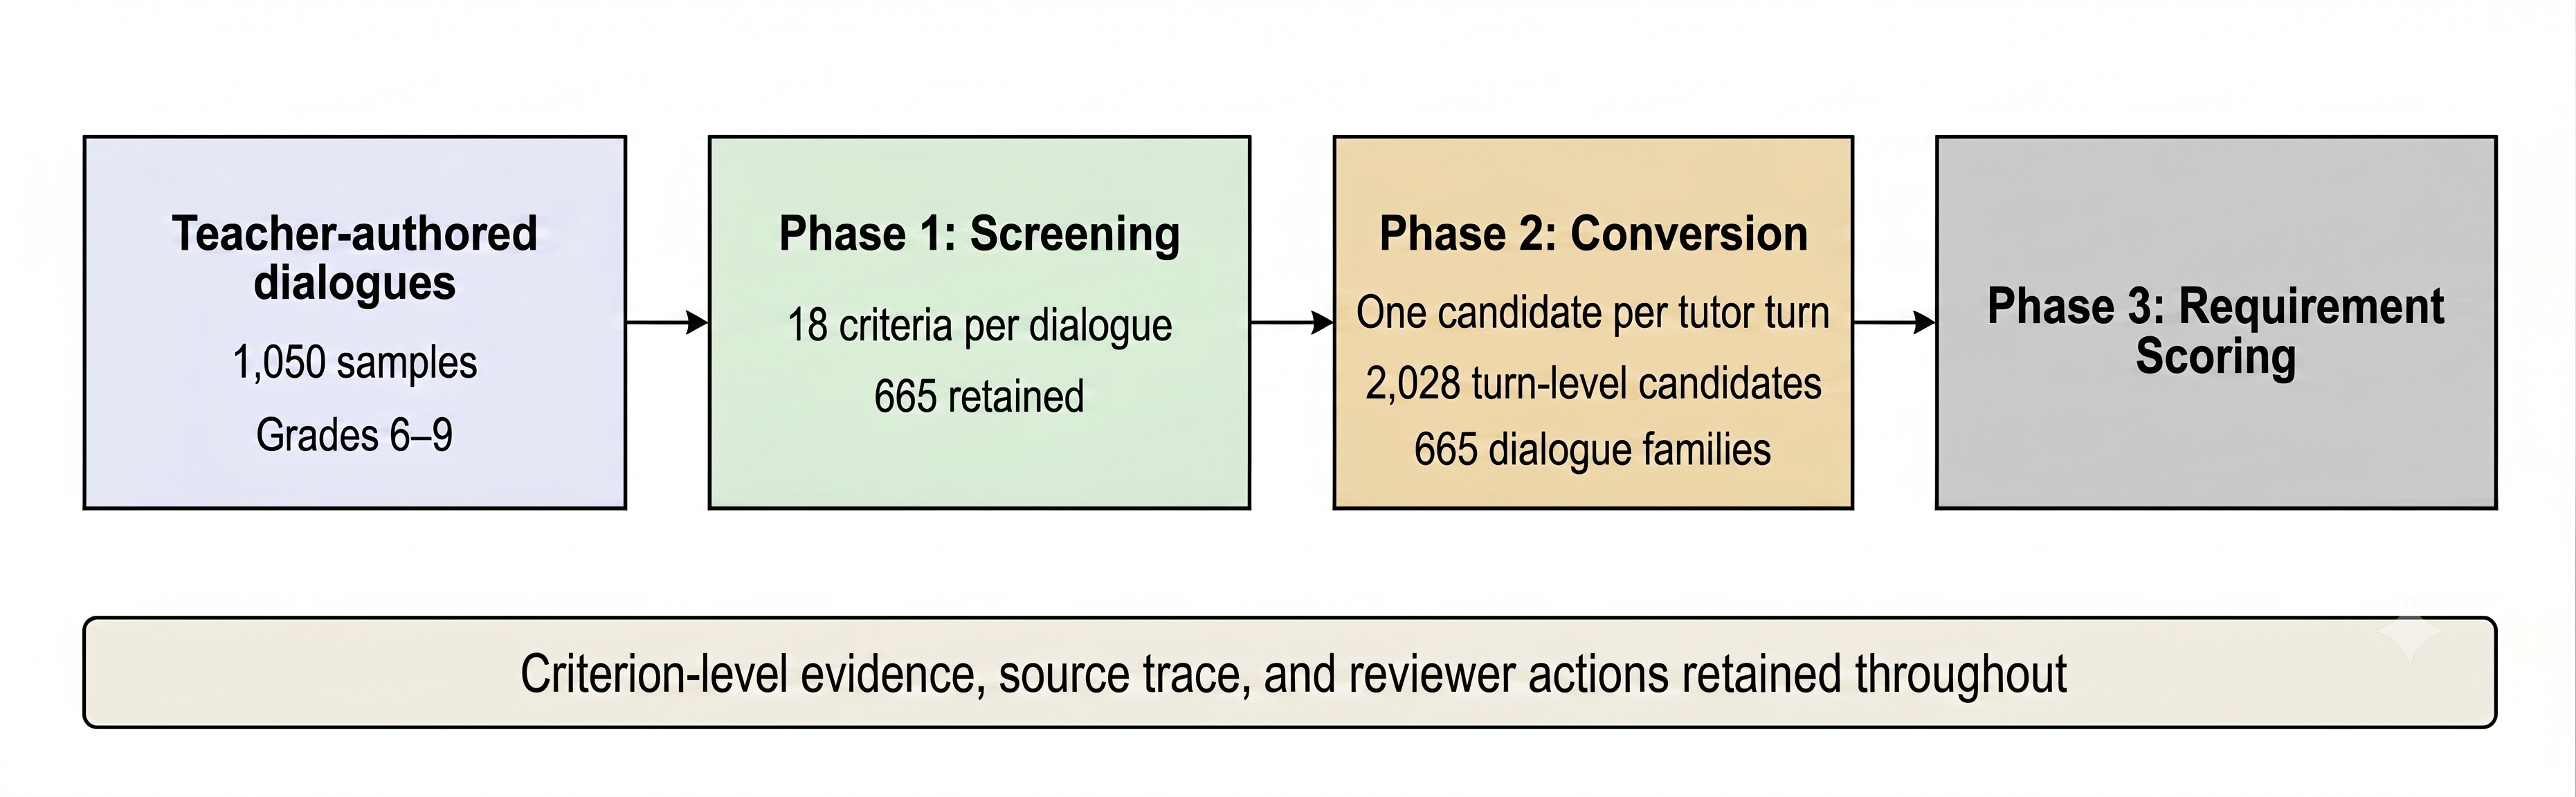
\includegraphics[width=0.8\textwidth]{figures/overall_pipeline.png}
\caption{Overview of the three-phase benchmark-construction pipeline. Phase~1
and Phase~2 provide complementary inputs to Phase~3.}
\label{fig:construction-pipeline}
\end{figure*}
}{}

\subsection{Phase 1: Screening Teacher-Authored Dialogues}

The construction process began with 1,050 teacher-authored Vietnamese
Informatics dialogues for Grades~6--9. Phase~1 was a screening procedure,
not a claim that a dialogue was already a final valid benchmark item.
Before auditing the dialogues, we prepared a curriculum-evidence layer from
the Vietnamese Informatics textbooks (SGK) and teacher guides (SGV) for
Grades~6--9. We normalized 154 OCR-derived Markdown units and split them into
2,750 traceable fragments. Each fragment retains its grade, material type,
lesson or page location, and a stable identifier. A rebuildable SQLite
full-text search (FTS) index supports metadata filtering followed by keyword
retrieval. During auditing, SGK fragments primarily ground lesson scope,
student questions, and topic consistency, whereas SGV fragments primarily
ground expected answers and explanations.

Phase~1 covered five audit areas at the overall audit-process level:
\begin{itemize}
    \itemsep0pt
    \item coverage;
    \item missing fields and formatting;
    \item consistency;
    \item duplicate and near-duplicate detection; and
    \item per-sample quality assessment.
\end{itemize}
Within this process, individual dialogues were assessed using an
18-criterion checklist organized into four criterion groups:
\begin{itemize}
    \itemsep0pt
    \item Structure (3 criteria);
    \item Consistency (7 criteria);
    \item Pedagogy (6 criteria); and
    \item Duplicate risk (2 criteria).
\end{itemize}
The five audit areas are therefore not five groups of the 18 criteria:
coverage is evaluated at batch level and does not create a criterion row for
every dialogue. Code handled mechanical checks such as required fields,
speaker labels, lesson mapping, coverage, and duplicate candidates. The
semantic and pedagogical audit was led by the dedicated
\texttt{hnmu-dialogue-auditor} specialist, instantiated with
\texttt{gpt-5.4-mini} at medium reasoning effort. The dialogues were divided
into disjoint lesson-based shards. For every sample, the specialist combined
the raw fields, retrieved SGK/SGV fragments, and HNMU cognitive-level and
scaffolding guidance to assess all 18 criteria independently. Each
sample--criterion record stores the decision, confidence, evidence fragment,
reason, and suggested reviewer action. Code then validated checklist
completeness, merged the shards, and applied the strict sample-level
aggregation rule below; the specialist did not directly assign the final
sample status.
% Figure~\ref{fig:phase1-workflow} shows the detailed workflow.

% \begin{figure*}[h]
% \centering
% 
\includegraphics[width=0.5\textwidth]{figures/phase_1_flow.png}
% \caption{Detailed Phase~1 workflow, including data intake, learning-resource
% preparation, criterion-level auditing, and strict sample-level aggregation.}
% \label{fig:phase1-workflow}
% \end{figure*}

We aggregated these criterion-level judgments with a strict rule:
\begin{itemize}
    \itemsep0pt
    \item \textit{Failed}: at least one criterion is labelled \textit{fail}.
    \item \textit{Need human review}: no criterion is labelled \textit{fail}
    and at least one criterion is labelled \textit{uncertain}.
    \item \textit{Pass}: every criterion is labelled \textit{pass} or
    \textit{not applicable}.
\end{itemize}
This rule produced 665 \textit{pass} dialogues, 382 dialogues requiring
human review, and 3 failed dialogues. Only the 665 \textit{pass} dialogues
were retained for candidate construction in Phase~3. Thus, Phase~1 is a
traceable eligibility filter
rather than proof that every retained dialogue is already a final valid
benchmark item.

For the 665 retained Phase~1 dialogues, one turn denotes one utterance
labelled \texttt{HS:} or \texttt{AI:}, not a student--tutor exchange.
Character length is computed from the utterance content after removing the
speaker label and colon; internal whitespace and line breaks remain included.
These statistics use \texttt{raw\_dialogue}, not \texttt{conversion\_dialogue}
or later Phase~1 recheck artifacts. Figure~\ref{fig:phase1-statistics}
summarizes the resulting distributions.

\begin{figure*}[h]
\centering
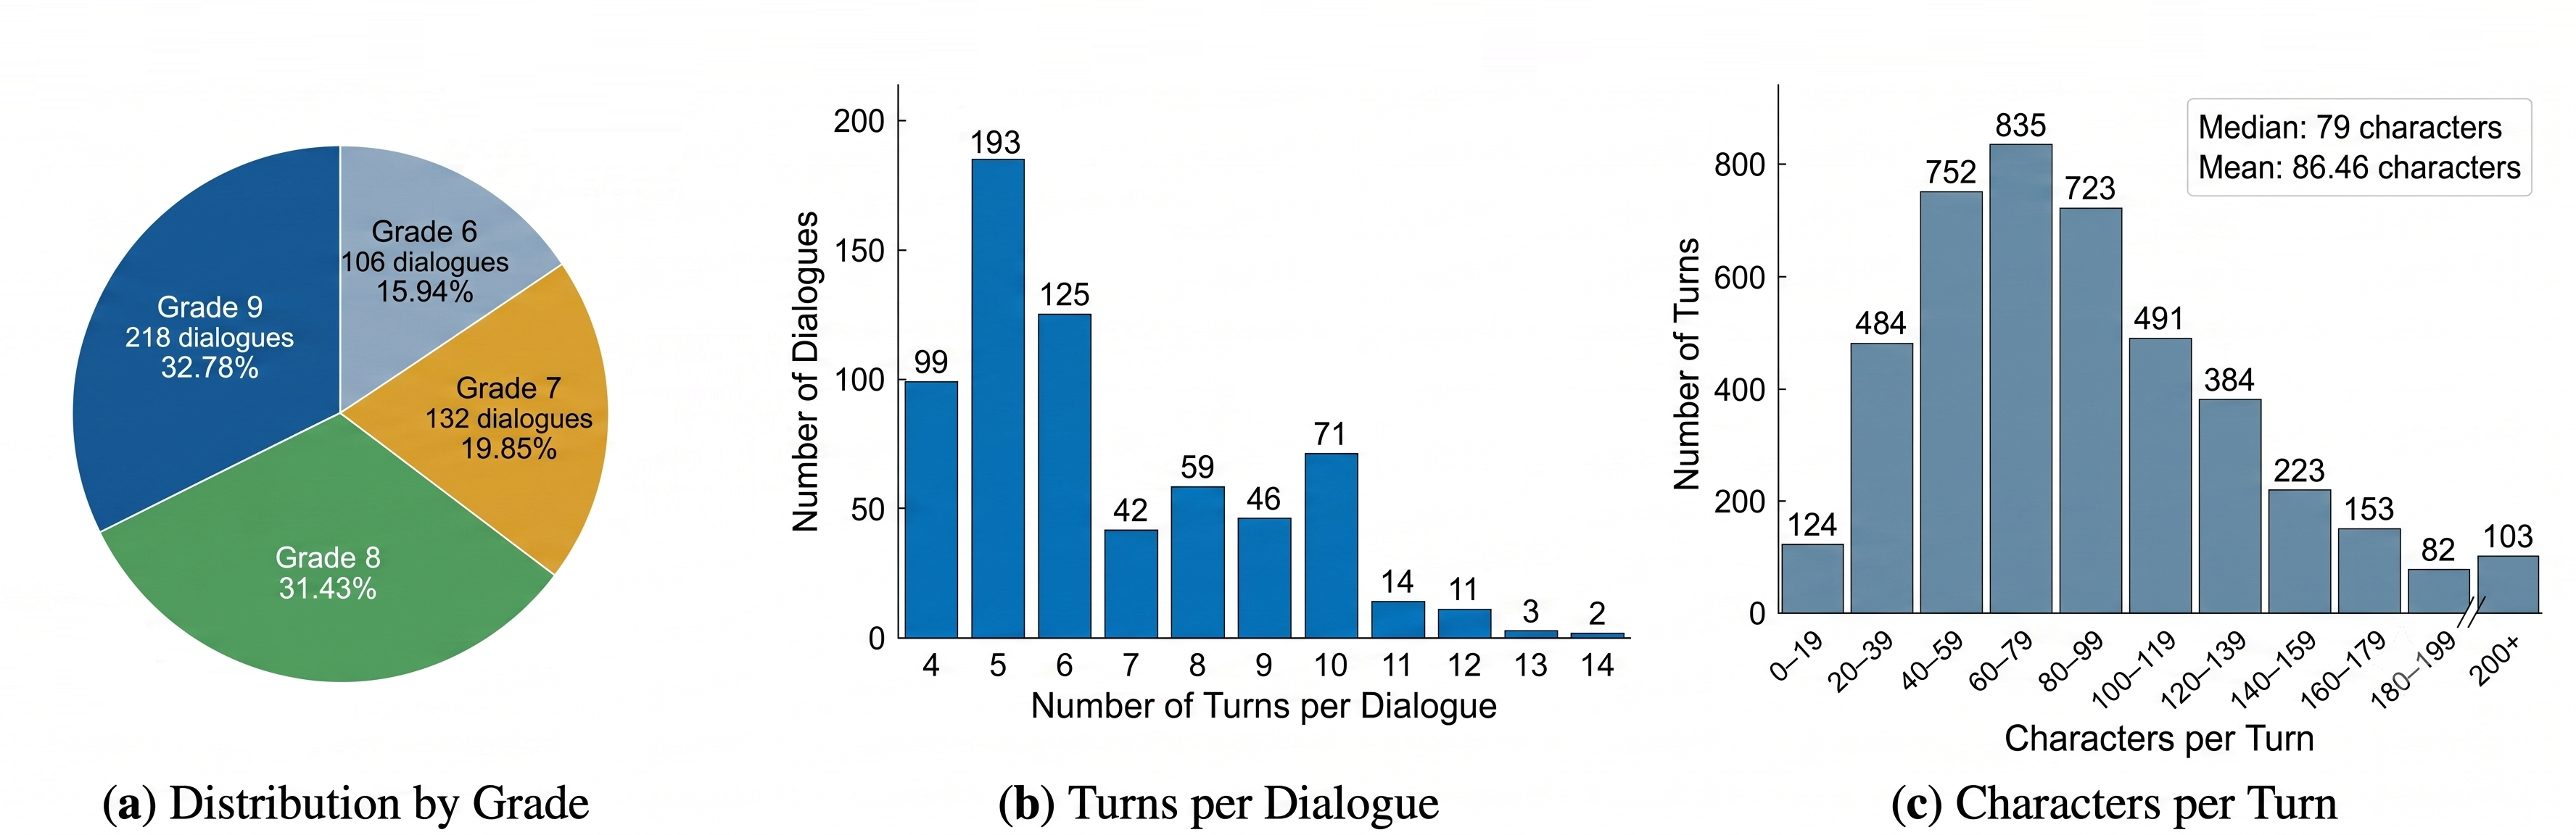
\includegraphics[width=1.0\textwidth]{figures/statistic.png}
\caption{Descriptive distributions of the 665 dialogues retained after
Phase~1: grade, number of turns per dialogue, and character length per turn.}
\label{fig:phase1-statistics}
\end{figure*}

Grades~8 and 9 account for 209 (31.43\%) and 218 (32.78\%) dialogues,
respectively, or 64.21\% together; the retained set is therefore more heavily
represented by the two upper grades. Grades~6 and 7 contribute 106 (15.94\%)
and 132 (19.85\%) dialogues. Dialogues range from 4 to 14 turns, with a
median of 6 and a mode of 5; 193 dialogues (29.02\%) contain 5 turns and
417 (62.71\%) contain 4--6 turns. Across 4,354 turns, 2,326 are student
turns and 2,028 are AI turns. Character length ranges from 7 to 294
(Q1=53, median=79, Q3=113; mean=86.46). The mean exceeding the median
indicates a moderate upper tail in turn length, and the median AI turn
length (108 characters) exceeds the median student-turn length (60).

\subsection{Phase 2: Pedagogical Measurement Foundation}

We distinguish pedagogical \emph{functions} from tutor \emph{quality
attributes}. The functional layer adopts Allison and Tharby's six
interrelated principles---Challenge, Explanation, Modelling, Practice,
Feedback, and Questioning---as operationalized for tutor-response evaluation
by KMP-Bench \cite{allison2015making,shi2026kmpbench}. They respectively
capture productive cognitive demand; conceptual clarification; demonstration
of application; opportunities for independent practice; response grounded in
learner work; and questions whose answers advance the interaction.

The capability layer was synthesized from the three tutoring benchmarks,
adaptive-scaffolding research, the HNMU tutoring method, and evidence-centered
assessment design. It comprises \textit{(i)} subject-matter accuracy and
grounding; \textit{(ii)} learner-state modelling; \textit{(iii)}
pedagogical-strategy selection; \textit{(iv)} scaffolding calibration;
\textit{(v)} diagnosis of errors, misconceptions, and missing prerequisites;
and \textit{(vi)} clear, supportive, age-appropriate communication
\cite{macina2025mathtutorbench,shi2026kmpbench,srinivasa2025tutorbench,
vandepol2010scaffolding,mislevy2003ecd}. Boundary analysis separates
learner-state description from causal diagnosis, and the choice of a
pedagogical means from the amount, timing, and transfer of support. The
principles later activate response-specific instructions and criteria; the
capabilities ensure that the overall rubric covers the qualities of an
effective tutor.

\subsection{Phase 3: From Raw Dialogues to Benchmark Data}

\subsubsection{Turn-level candidate construction}
The 665 retained dialogues were converted deterministically by treating every
tutor turn as a possible target. The initial student turn becomes the first
prompt; all intervening utterances retain their student or tutor role as
conversation history; and the selected tutor turn becomes the reference
response. Turns after the target are excluded. The teacher-provided answer is
kept separately as subject-matter grounding. This policy produces 2,028
candidates across 665 dialogue families, including multiple history depths
from the same source dialogue. A one-to-one trace records the source file,
row, target-turn position, and any approved correction, while family IDs
prevent candidates from the same dialogue being split across evaluation
partitions.

\subsubsection{LLM-assisted principle assignment and filtering}
For each candidate, Gemini~3.5~Flash receives the grade, lesson, target
position, Bloom level, student prompt, role-preserving history, source
question, and teacher-provided answer. The reference response is deliberately
excluded so that the criteria are not selected from the strengths of the
response against which a model will later be compared. The scorer rates the
necessity of each principle on a five-point scale: 1 denotes irrelevant or
counterproductive; 2 weakly related; 3 a valid but optional strategy; 4
required for a good response; and 5 essential to the main pedagogical need.
Code, rather than the LLM, selects every principle scoring at least 4 and
performs schema validation, thresholding, semantic linting, and routing.

\subsubsection{Eligible benchmark pool and descriptive statistics}
The full scoring run contains 12,168 principle scores for all 2,028
candidates. Deterministic gates place 1,400 candidates in
\texttt{eligible\_without\_plan03\_review}, 628 in targeted UET review, and
none in a structurally blocked state. The eligible pool spans 655 families:
443 candidates require one principle, 866 require two, and 91 require three.
It contains 631 candidates without history and 769 with non-empty history.
Table~\ref{tab:eligible-pool} reports grade and principle incidence; because a
candidate can require multiple principles, principle counts do not sum to
1,400.

\begin{table}[t]
\caption{Composition of the 1,400-candidate eligible pool.}
\label{tab:eligible-pool}
\centering
\small
\begin{tabular}{lrr@{\hspace{7pt}}lrr}
\hline
\textbf{Grade} & \textbf{N} & \textbf{\%} &
\textbf{Principle} & \textbf{N} & \textbf{\%} \\
\hline
6 & 193 & 13.8 & Challenge & 8 & 0.6 \\
7 & 280 & 20.0 & Explanation & 863 & 61.6 \\
8 & 412 & 29.4 & Modelling & 93 & 6.6 \\
9 & 515 & 36.8 & Practice & 27 & 1.9 \\
 & & & Feedback & 806 & 57.6 \\
 & & & Questioning & 651 & 46.5 \\
\hline
\end{tabular}
\end{table}

\section{Evaluation Framework}

Following the KMP-Dialogue structure \cite{shi2026kmpbench}, our framework
separates tutor-input preparation, criterion construction, and blind
pairwise assessment.

\subsection{Context Loading and Tutor-Response Generation}

The tutor model receives a system instruction containing its Vietnamese
secondary-school Informatics tutoring role, grade, lesson, source task, a
common tutoring instruction, and the exact set of required principles.
The dialogue itself is sent through the provider's native multi-turn
interface: the initial student prompt and subsequent student turns use the
\texttt{user} role, while prior tutor turns use the
\texttt{assistant}/\texttt{model} role. The final message is always the
student turn to be answered. Candidate IDs, principle scores, criteria,
learning-resource fragments, the teacher-provided answer, and the reference
response are not shown to the tutor model.

\subsection{Two-Tier Rubric Construction}

Six tutor capabilities provide a coverage map for four common criteria:
\textit{(i)} subject-matter accuracy and verifiability; \textit{(ii)}
alignment with the learner's state and immediate goal; \textit{(iii)}
calibrated support that preserves meaningful learner work; and
\textit{(iv)} clear, respectful, age-appropriate communication. Each of the
six principles contributes three additional criteria that measure only its
incremental pedagogical function. A candidate requiring \(n\) principles is
therefore evaluated with \(4 + 3n\) criteria. This produces a stable common core while adapting the remaining
criteria to the pedagogical demands of the candidate.

We additionally define six serious-error gates: wrong subject matter,
fabricated grounding, reinforcement of a misconception, bypassing the
learning process, harmful or demeaning content, and failure to address the
learner's need. These gates are not scored as extra criteria. Instead, each
gate can adjust only the intersection between the criteria it affects and the
criteria active for the candidate, preventing duplicate penalties.

\subsection{Blind Pairwise Judging and Score Aggregation}

The judge receives the same dialogue context, the source question,
teacher-provided answer, relevant textbook/teacher-guide fragments, all
applicable criteria, and two anonymous responses: the generated tutor
response and the teacher-authored reference. Their order is randomized with a
fixed seed and restored only after judging. In one call, the judge returns a
Win, Tie, or Lose decision for every applicable criterion, detects serious
errors independently in both responses, and provides a separate holistic
judgment. The comparison explicitly permits a generated response to
outperform the reference.

Let \(W_r,T_r,L_r\) be the numbers of Win, Tie, and Lose judgments for
criterion \(r\). Its win rate is
\[
 A_r = \frac{W_r}{W_r+T_r+L_r},
\]
so a Tie is retained in the denominator rather than converted to 0.5.
General-Level Accuracy is the mean of the four common \(A_r\) values, while
Principle-Level Accuracy for principle \(p\) is the mean of its three
criteria. Overall Accuracy averages General-Level Accuracy and the macro mean
of the six Principle-Level scores. The holistic Win rate is reported
separately. All analyses retain the full Win/Tie/Lose distribution and report
both candidate-level and dialogue-family-level aggregates.

\section{Experiments and Analysis}

\subsection{Experimental Setup}

The current evaluation pool comprises the 1,400 candidates that passed the
Phase~3 gates. The tutor panel contains \textit{(i)} Gemini~3.5~Flash, a
closed general-purpose model accessed through Vertex AI; and \textit{(ii)}
Llama~4~Maverick, an open-weight general-purpose model accessed through
Vertex AI Model-as-a-Service. A third configuration applies a
LearnLM-oriented educational system instruction to the same
Gemini~3.5~Flash base model; it is analyzed as a prompt ablation, not as an
independent model. A specialized tutoring checkpoint was considered
separately but was not included before passing deployment and Vietnamese
response checks.

For Gemini target generation, sampling parameters are omitted,
\texttt{thinking\_level=MEDIUM}, hidden thoughts are not returned, and seed
20260728 is fixed. The initial output cap is 1,024 tokens; only responses
terminated by the token limit are retried with a higher cap. Llama uses the
same 1,024-token initial cap and omits sampling parameters. All requests store
the exact system instruction, native message sequence, model configuration,
finish reason, token usage, and content hashes.

Gemini~3.5~Flash serves as the primary blind pairwise judge with
\texttt{thinking\_level=MEDIUM}, a fixed seed, and an 8,192-token output
cap. One judge call evaluates all applicable criteria and the holistic
comparison for a candidate--model pair. Results in which Gemini is both tutor
and judge are reported separately to expose possible same-model bias.

\subsection{Reported Measures}

For each tutor configuration, we report \textit{(i)} the win rates and full
Win/Tie/Lose distributions for the four common criteria; \textit{(ii)} six
Principle-Level Accuracy scores; \textit{(iii)} General-Level Accuracy;
\textit{(iv)} Overall Accuracy; \textit{(v)} holistic judgment Win rate; and
\textit{(vi)} serious-error incidence and the number of criterion decisions
changed by an error gate. Results are stratified by grade, principle, history
availability, and dialogue family. The pool statistics in
Table~\ref{tab:eligible-pool} show that Explanation, Feedback, and Questioning
dominate, whereas Challenge and Practice are rare; principle-level reporting
is therefore necessary in addition to a single overall score.

\section{Discussion and Limitations}
\textit{To be completed.}

\section{Conclusion}
\textit{To be completed.}

\bibliographystyle{IEEEtran}
\bibliography{references}

\end{document}
